The concept of the adjacency/proximity matrix $\mathbf W$, first introduced by  Cressie (1993) in areal data analysis, is pivotal to reflect the dependence among nearby locations.
The entries $ w_{ij}$ in the adjacency matrix describe the connection between location $ i$ and $j$ in some fashion.
Typically, one builds the adjacency matrix based on either a distance or a binary status.
For instance, one can define $w_{ij} = 1$ if $i$ and $j$ share some common boundary and 0 otherwise.
Alternatively, $w_{ij}$ could reflect ``distance'' between units.
Further modifications can be made as well.
For instance, we could set $w_{ij} = 1$ for all $i$ and $j$ within a specified distance.
Or,  for a given $i$, we could define $w_{ij} = 1$ if $j$ is one of the $K$ nearest (in distance) neighbors of $i$.
In the context of our study, we define the adjacency matrix based on the watershed information since it serves as an indicator of flood activity and its domain.
Specifically, if two locations $ i$ and $ j$ are within the same watershed, then $ w_{ij} = 1$ and $ w_{ij} = 0$ otherwise. \hl{Note that this choice reflects the river network connections.}\\

A watershed is an area of land where rainfall accumulates and drains off into a river, bay or other body of water (Betson et al., 1964).
Other terms used interchangeably with watershed are drainage area, catchment basin and water basin.
The watersheds have different scales and the hierarchy is reflected by HUC system.
For instance, an area indexed by a two-digit code is composed of several smaller four-digit basins.
There are six levels in the hierarchy, represented by hydrologic unit codes from two to twelve digits long, called regions, subregions, basins, subbasins, watersheds, and subwatersheds (Seaber et al., 1987).
Figure~\ref{fig:size_comp} illustrates all the six-digit and eight-digit hydrological units that are located fully or partially in South Carolina.

\begin{figure}[htbp]
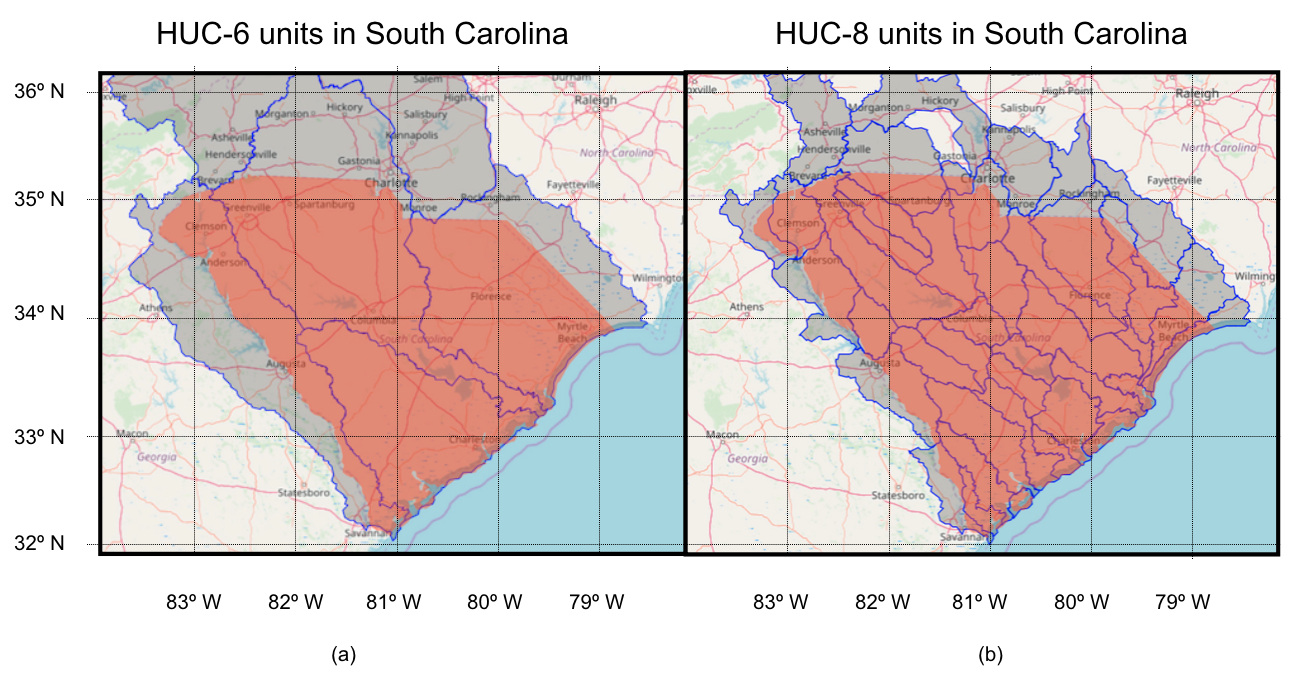
\includegraphics[width=1\textwidth]{../images/huc_units_in_sc.png}
\caption{\hl{An area is counted even if only part of it is inside the state border. Six-digit hydrological units are used to build our predictive model. The red shaded area indicates the territory of the state of South Carolina.}}
\label{fig:size_comp}
\end{figure}

Notably, basins (areas indexed by a \hl{HUC-6} code) appear to be an appropriate granularity when we investigate the watersheds in South Carolina, since these hydrological areas are neither too dense nor sparse in terms of data points.
Table~\ref{fig:real_huc} summarizes the unique locations in our data set in each HUC region.
Since the HUC regions do not exactly match state borders, we retain the regions in which the majority of observations are located in South Carolina, namely, Savannah, Santee, Edisto-South Carolina Coastal and Lower Pee Dee (Figure~\ref{fig:size_comp} left panel, clockwise from left to right) in terms of HUC-6 regions.
 Note that the Savannah,  Lower Pee Dee and Santee watersheds are not exclusively located in South Carolina, as there are initially formed and originated from Georgia and North Carolina.
 We consider these locations outside South Carolina as part of our data set as well when collecting flood gage height and other variables, since they are integral parts of the watersheds and contribute to the runoff generation, as well.\\

\begin{table*}[htbp]
\centering
\begin{tabular}{|l|l|}
\hline
Name & Count\\\hline
Santee & 108\\\hline
Lower Pee Dee&24\\ \hline
Savannah & 21\\ \hline
Edisto-South Carolina Coastal &19\\ \hline
\end{tabular}
\caption{The counts of available locations in each HUC-6 region. }
\label{fig:real_huc}
\end{table*}

Alternatively, to define the proximity matrix, one can use a \emph{river basin} system as well, which is a product of the first watershed planning activities in 1970s by the state of South Carolina.
According to the river basin system, eight mutually exclusive areas are defined: Broad River, Savannah River, Pee Dee River, Santee River, Catawba River, Catawba River, Saluda River, Edisto River and Salkehatchie River.
 However, we prefer the watershed system since it is not constrained by state borders.
 Furthermore, based on the river basin  segmentation, some river basins, e.g., Salkehatchie, contain as few as two unique observing stations.
 Such sparsity might lead to less stable parameter estimates.

\begin{figure}[htbp]
\begin{center}
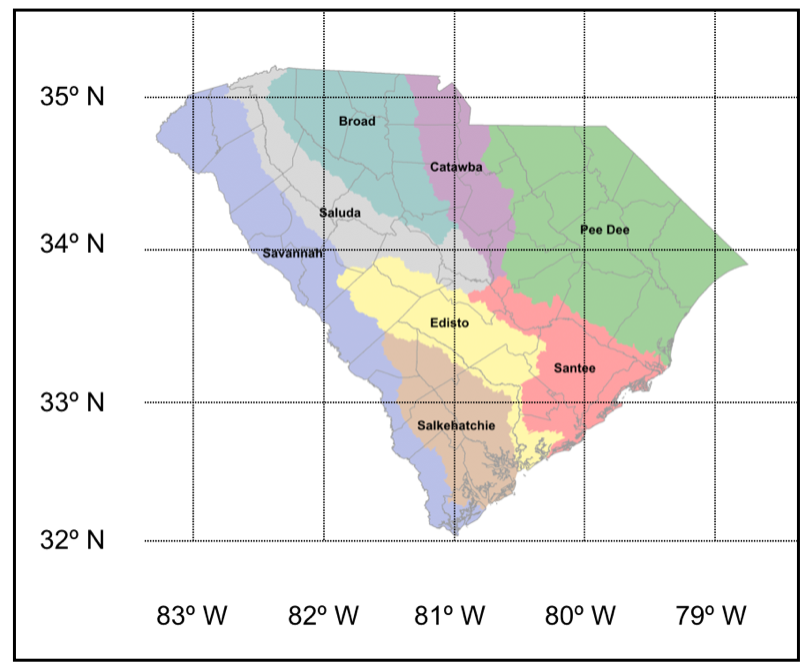
\includegraphics[width=0.5\textwidth]{../images/basin_areas_in_sc.png}
\caption{\hl{Major basins in South Carolina}}
\label{fig:river_basins_}
\end{center}
\end{figure}